\documentclass[11pt]{article}
\usepackage[margin=1.05in]{geometry}
\usepackage{amsmath,amssymb,amsthm,mathtools}
\usepackage{booktabs,microtype,xcolor}
\usepackage[shortlabels]{enumitem}
\usepackage[colorlinks=true,linkcolor=blue!45!black,citecolor=blue!45!black,urlcolor=blue!45!black]{hyperref}
\hypersetup{pdftitle={Vertex crossings and boundary regimes in a symmetric Markov multinomial model},pdfauthor={Arjun Pemmasani}}
\newtheorem{theorem}{Theorem}[section]
\newtheorem{lemma}[theorem]{Lemma}
\newtheorem{proposition}[theorem]{Proposition}
\newtheorem{corollary}[theorem]{Corollary}
\theoremstyle{definition}
\newtheorem{definition}[theorem]{Definition}
\newtheorem{example}[theorem]{Example}
\theoremstyle{remark}
\newtheorem{remark}[theorem]{Remark}
\newcommand{\Z}{\mathbb Z}
\newcommand{\E}{\mathbb E}
\newcommand{\Prob}{\mathbb P}
\newcommand{\Var}{\operatorname{Var}}
\newcommand{\Cov}{\operatorname{Cov}}
\title{Vertex crossings and boundary regimes\\
 in a symmetric Markov multinomial model}
\author{Arjun Pemmasani}
\date{September 22, 2026\\[0.5ex]
 \small Unsubmitted draft; held for further review}
\begin{document}
\maketitle

\begin{abstract}
We study occupation counts of a stationary Markov chain that repeats its
current state with probability $p$ and otherwise chooses uniformly among
$d-1$ alternatives. For fixed $d$, we compare the probability of an individual
count vector with that of a vertex, where every visit is to one state.
A positive refresh expansion gives a relative Bessel approximation uniform
over all positive compositions, including vectors approaching simplex
boundaries. We obtain explicit crossing expansions for balanced faces and
interior compositions, and a rare-coordinate crossover at
$N/(\log N)^2$ when at least two coordinates are macroscopic. Near a vertex,
a product of finite Laguerre polynomials determines the leading crossing
uniformly for arbitrary rare counts with total $A=o(b)$, where $b$ is the
dominant count; the relative root error is
$O_\ell(\sqrt{(A+1)/b})$. This root approximation can hold even when its
corresponding probability approximation diverges. We also determine
spatial superlevel volumes and construct weak occupation fields that make
every support size optimal in succession. Exact laws and ordinary normal
limits are included as background. The proposed contributions are the
uniform moving-parameter estimates and their boundary and modal
consequences; historical priority remains to be established.
\end{abstract}

\section{Introduction}

A symmetric persistent chain provides a simple model in which the most
likely occupation vector changes from a vertex to the interior as the
persistence decreases. The comparison involves the probability of one
specific vector, rather than the aggregate probability of a face. It is
especially sensitive to coordinates that are small relative to the total
number of visits. This paper studies those crossing locations for a fixed
number of states, including count vectors approaching a vertex at
arbitrary rates.

The model is a multistate version of the Galton-board process in Kagey's
Problem 131~\cite{kagey131}. The binary analysis and its free/periodic
boundary comparison are developed in the unpublished
companion~\cite{companion}. Here we state the multistate model explicitly
and prove all estimates needed for the multistate results; no theorem from
the companion is required for a proof in this paper. In geometric terms,
the occupation vectors index the bins of a simplex board with fixed global
directions and uniform switching. Other rules at physical boundaries can
define different processes.

Our main estimates address three regimes. On a fixed simplex face, the
balanced crossing lies in the common window
$Nu=\log N-\tfrac12\log\log N+O(1)$, with explicit constants depending on
its support size. A relative Bessel bound uniform over every positive
composition resolves the transition when additional coordinates have size
$N/(\log N)^2$. Finally, if one count is $b$ and the remaining counts have
total $A=o(b)$, a single polynomial equation gives the crossing with
relative error $O_\ell(\sqrt{(A+1)/b})$, uniformly over their individual
sizes. The last assertion remains valid in a regime where the associated
probability approximation is not uniform. The modal consequences include
spatial superlevel volumes and an explicit weak field for which all
support sizes occur successively.

\paragraph{Relation to established results.}
The underlying law belongs to Markov multinomial theory
\cite{wangyang1995,wangtang2003}. The exact finite sum and the ordinary
normal limit recorded below are background, not novelty claims. The
original Wang--Yang article has not been obtained; its bibliographic
information is reported through Wang and Tang, and comparison with its
full text remains part of the priority review.
General continuous-time occupation densities on visited simplex faces
are also established~\cite{brydges2007}. The square-root composition
quantity appearing below is classical: if $Q$ is the complete-graph
continuous-time generator with off-diagonal entries one, then its
symmetric occupation rate is
\[
 I_Q(\alpha)=-\langle\sqrt\alpha,Q\sqrt\alpha\rangle
 =d-\left(\sum_i\sqrt{\alpha_i}\right)^2.
\]
Thus the exponent $(\sum_i\sqrt{\alpha_i})^2-1$ is the difference
between the vertex rate and the rate at $\alpha$. We do not claim this
rate function as a new result. Standard Bessel expansions are taken from
\cite{dlmf}; all discrete comparison estimates and root inversions used
here are proved explicitly. The proposed contribution is their uniform
control in moving persistence regimes and the resulting boundary and
modal statements. The literature search has not established historical
priority, and this draft is held for further mathematical and
bibliographic review.

\paragraph{Organization and scope.}
Section~\ref{sec:multistate-model} gives the exact law, elementary
estimates, and fixed-persistence covariance and normal limit.
Section~\ref{sec:simplex-thresholds} proves the face crossings and
balancing theorem. Sections~\ref{sec:frontier-boundary}
and~\ref{sec:vertex-completion} treat boundary coordinates and the
uniform near-vertex law. Section~\ref{sec:frontier-modes} treats
superlevel sets and weak fields. The results do not give every finite-size
global mode or cover a growing number of states. A finite-size example
shows why a vertex/full-center dichotomy cannot hold without qualification.

\section{The model and exact formulas}\label{sec:multistate-model}

Fix $d\ge2$ and let $(X_j)_{j\ge1}$ be a Markov chain on
$\{1,\ldots,d\}$. The initial state is uniform.
At each subsequent step the chain repeats its state with probability
$p\in[0,1]$ and moves to each other state with probability
$r=(1-p)/(d-1)$. Put $q=1-p$ and
$\sigma=p-r=(dp-1)/(d-1)$. Let $K_N=(K_{N,1},\ldots,K_{N,d})$
be the occupation vector over $N$ visits, and write
$P_N(k)=\Prob(K_N=k)$. For a word $w$ of length $N\ge1$ with
$j$ changes, its probability is $d^{-1}p^{N-1-j}r^j$.
The vertex probability is $V_N=p^{N-1}/d$.
For $p>0$ put $u=r/p$; for a positive vector
$n=(n_1,\ldots,n_k)$ with total $N$, write
\[
 S_n(u)=\frac{P_N(n_1,\ldots,n_k,0,\ldots,0)}{V_N}
 =\sum_j W_n(j)u^j,
\]
where $W_n(j)$ counts words on the specified $k$ states with these
occupations and $j$ changes. The ratio is independent of the ambient
number $d$ once the positive coordinates are fixed.
Set $P_0(0,\ldots,0)=1$ separately.

\begin{proposition}[$d$ directions]\label{prop:dgf}
Let $P_N(k_1,\dots,k_d)$ be the probability that direction $i$ is taken $k_i$ times. Put
$\sigma=p-\frac{q}{d-1}=\frac{dp-1}{d-1}$ and $\mathcal R=\sum_{i=1}^d\frac{x_it}{1-\sigma x_it}$. Then
\[
\sum_{N\ge0}\sum_{k_1+\dots+k_d=N}P_N(k_1,\dots,k_d)\,x_1^{k_1}\cdots x_d^{k_d}\,t^N
=1+\frac{\mathcal R/d}{1-\frac{q}{d-1}\mathcal R}.
\]
\end{proposition}

\begin{proof}
Let $F_i$ be the generating function of words ending in state $i$, and $S=\sum_iF_i$.
Conditioning on the last bounce, $F_i=x_it\bigl(\tfrac1d+pF_i+\tfrac{q}{d-1}(S-F_i)\bigr)$, that is
$F_i(1-\sigma x_it)=x_it\bigl(\tfrac1d+\tfrac{q}{d-1}S\bigr)$. Summing over $i$ gives
$S=\mathcal R\bigl(\tfrac1d+\tfrac{q}{d-1}S\bigr)$, and the generating function is $1+S$.
\end{proof}

For $d=2$, setting $x_1=x$ and $x_2=1$ gives the binary generating function studied in the companion~\cite{companion}.

\begin{proposition}[finite bin probabilities in $d$ directions]\label{prop:dpmf}
Put $r=q/(d-1)$ and $\sigma=p-r$. For $N\ge1$, let $k=(k_1,\ldots,k_d)$ have
nonnegative integer coordinates summing to $N$, and put $H=\{i:k_i>0\}$. Sum over
$m_i=0$ for $i\notin H$ and $1\le m_i\le k_i$ for $i\in H$, and set $M=\sum_i m_i$.
Then
\[
P_N(k)=\frac1d\sum_m\frac{M!}{\prod_i m_i!}\,
r^{M-1}\sigma^{N-M}\prod_{i\in H}\binom{k_i-1}{m_i-1}.
\]
All exponents are nonnegative, and $0^0=1$. Set $P_0(0,\ldots,0)=1$ separately.
\end{proposition}
\begin{proof}
With $z_i=x_it$, Proposition~\ref{prop:dgf} becomes the formal power series
\[
1+\frac1d\sum_{M\ge1}r^{M-1}
\left(\sum_i\frac{z_i}{1-\sigma z_i}\right)^M.
\]
Expand by the multinomial theorem and use, for $k\ge m\ge1$,
\[
[z^k]\left(\frac{z}{1-\sigma z}\right)^m
=\binom{k-1}{m-1}\sigma^{k-m}.
\]
For $m=0$ only $k=0$ contributes. Multiplying the coefficients proves the formula.
\end{proof}

At $d=3$ this is a triple sum, with the support convention covering edge bins.
At $p=1/d$, $\sigma=0$ and only $M=N$ survives, giving the ordinary multinomial law.
At $p=1$, only $M=1$ survives, giving mass $1/d$ at each $Ne_i$.
The formula is valid also at $p=0$; for $\sigma<0$ its terms can cancel, so dynamic
programming or exact arithmetic is preferable numerically. This geometry assumes fixed global
directions and uniform switching to the other directions; a different physical boundary or
orientation rule need not have this law.



\subsection{Elementary bounds used below}

For $x\ge0$, the modified Bessel function used here is
\[
 I_1(x)=\sum_{j\ge0}\frac{(x/2)^{2j+1}}{j!(j+1)!}.
\]
Its coefficients give $I_1(x)\le\sinh x\le e^x$.
We also use the standard expansion~\cite[Eq.~10.40.1]{dlmf}
\[
 I_1(x)=\frac{e^x}{\sqrt{2\pi x}}
 \left(1-\frac{3}{8x}+O(x^{-2})\right),\qquad x\to\infty.
\]
The Laguerre--Bessel comparison needed at boundaries is proved in
Lemma~\ref{lem:uniform-laguerre-bessel}; it is not imported from the
binary companion.

\begin{lemma}[clipped product deficit]\label{lem:clipped-product}
For any finite list of nonnegative real numbers $t_1,\ldots,t_m$,
with $(x)_+=\max(x,0)$,
\[
 0\le1-\prod_{j=1}^m(1-t_j)_+\le\sum_{j=1}^m t_j.
\]
\end{lemma}
\begin{proof}
If some $t_j\ge1$, the product is zero and the sum is at least one.
Otherwise all factors lie in $[0,1]$ and induction follows from
$1-(1-a)(1-b)=a+b-ab\le a+b$. The empty product gives equality.
\end{proof}

\subsection{Covariance and the fixed-persistence normal limit}

The following formulas are recorded for comparison with the moving
regimes studied later. Their fixed-$p$ normal limit is not a local
approximation for individual occupation probabilities when $p$ depends
on $N$.

\begin{remark}[covariance and the tetrahedral case]\label{rem:tetra}
For the board with $d$ directions of Proposition~\ref{prop:dgf} let $K_a$ be the number of bounces in
direction $a$. The direction chain has transition matrix $\sigma I+(1-\sigma)\tfrac1dJ$ with $J$ the
all-ones matrix, so the indicator of direction $a$ at time $i$ and of direction $b$ at time $i+m$ have
covariance $\sigma^m\bigl(\tfrac{\delta_{ab}}d-\tfrac1{d^2}\bigr)$. Summing over the
two time indices and evaluating the finite geometric sum gives
\[
\Cov(K_a,K_b)=\Bigl(\frac{\delta_{ab}}d-\frac1{d^2}\Bigr)
\Bigl(N\,\frac{1+\sigma}{1-\sigma}-\frac{2\sigma(1-\sigma^N)}{(1-\sigma)^2}\Bigr),
\qquad \frac{1+\sigma}{1-\sigma}=\frac{d-2+dp}{d\,(1-p)} .
\]
These formulas hold for $p<1$; at $p=1$ the covariance is
$N^2(\delta_{ab}/d-1/d^2)$. The asymptotic multiplier of the multinomial covariance is
$(d-2+dp)/(d(1-p))$, which is $(1+3p)/(3(1-p))$ for the tetrahedron.
\end{remark}

\begin{theorem}[simplex normal limit]\label{thm:dclt}
Let $d\ge3$ and $0\le p<1$, or $d=2$ and $0<p<1$. Set
\[
\pi=(1/d,\ldots,1/d),\quad C=\frac1d I-\frac1{d^2}J,
\quad c=\frac{1+\sigma}{1-\sigma}=\frac{d-2+dp}{d(1-p)}.
\]
Then $(K_N-N\pi)/\sqrt N$ converges in distribution to $\mathcal N_d(0,cC)$.
This Gaussian is supported on the sum-zero hyperplane and is nondegenerate there.
\end{theorem}
\begin{proof}
Let $\Pi=\mathbf1\pi$ and $T=\sigma I+(1-\sigma)\Pi$. Fix a real vector $a$ and
put $f_i=a_i-d^{-1}\sum_j a_j$, so $\pi f=0$ and $Tf=\sigma f$.
For $D(t)=\operatorname{diag}(e^{itf_i})$ and $B(t)=TD(t)$, stationarity gives
\[
\E\exp\left(it\sum_{j=1}^N f(X_j)\right)
=\pi D(t)B(t)^{N-1}\mathbf1.
\]
At zero, $B(0)=T$ has the simple eigenvalue $1$ and all other eigenvalues equal
$\sigma$, with $|\sigma|<1$. Analytic perturbation gives an eigenvalue $\lambda(t)$
and right eigenvector $h(t)$ with $\lambda(0)=1$, $h(0)=\mathbf1$ and $\pi h(t)=1$.
The complementary spectral part is uniformly exponentially small for sufficiently small
$t$: choose a circle of radius $\eta<1$ enclosing the complementary spectrum but not
$\lambda(t)$ and use the resolvent formula for matrix powers. Thus the characteristic
function equals $b(t)\lambda(t)^{N-1}+O(\eta^N)$ with $b(t)\to1$.

Differentiate $Bh=\lambda h$ at zero. Since $B'(0)=iT\operatorname{diag}(f)$,
\[
\lambda'(0)=0,\qquad (I-T)h'(0)=i\sigma f,
\qquad h'(0)=\frac{i\sigma}{1-\sigma}f.
\]
Differentiating again and multiplying by $\pi$ gives
\[
\lambda''(0)=\pi B''(0)\mathbf1+2\pi B'(0)h'(0)
=-\frac{1+\sigma}{1-\sigma}\pi(f^2)=-c\,\pi(f^2).
\]
Hence $\lambda(t)=1-c\pi(f^2)t^2/2+O(t^3)$. Substitute $t=s/\sqrt N$ to obtain
the scalar normal characteristic function with variance $c\pi(f^2)=ca^{\mathsf T}Ca$.
L\'evy's theorem and the Cram\'er--Wold device give the result.
\end{proof}

For $d=3$ the first two centered coordinates have limiting covariance
\[
\frac{1+3p}{27(1-p)}\begin{pmatrix}2&-1\\-1&2\end{pmatrix};
\]
the third is minus their sum. Unlike the binary case, $p=0$ is included for $d\ge3$.
At $d=2,p=0$ bounded alternation gives the zero limit after division by $\sqrt N$.
At $p=1$ the centered sequence on this scale is not tight. This theorem asserts weak
convergence, not a local approximation for individual bin probabilities.



\section{Face-center thresholds on a simplex}\label{sec:simplex-thresholds}

We retain the symmetric $d$-direction model of Proposition~\ref{prop:dgf}:
the initial direction is uniform, a repeat has probability $p$, and each specified
change has probability $r=(1-p)/(d-1)$. Other ways of modeling a tetrahedral
board ($d=3$) give different laws, which we do not treat.
For $2\le k\le d$ and $N\ge k$, let $C_{N,k}(p)$ denote the probability of
one \emph{balanced face bin}: its $k$ positive coordinates differ by at most
one, and its other coordinates vanish. All such bins have the same probability.
Let $V_N(p)=p^{N-1}/d$ be the probability of one vertex bin, and put
\[
u=\frac{1-p}{(d-1)p},\qquad
a_k=\frac12\log(4\pi)-\frac{k+1/2}{k-1}\log k.
\]
The ratio $C_{N,k}/V_N$, viewed as a function of $u$, depends on $k$ and $N$
but not on the ambient number $d$ of directions.

\begin{theorem}[face-center crossings]\label{thm:simplex-crossing}
For every $2\le k\le d$ and $N\ge k$, there is exactly one
$p=p_{N,k}^{(d)}\in(0,1)$ for which $C_{N,k}(p)=V_N(p)$.
The face center is more likely below this persistence and less likely above it.
The sequence $p_{N,k}^{(d)}$ is strictly increasing in $N$, and
\[
p_{k,k}^{(d)}=\frac1{1+(d-1)(k!)^{-1/(k-1)}}.
\]
Writing $L=\log N$ and
$u_{N,k}=(1-p_{N,k}^{(d)})/((d-1)p_{N,k}^{(d)})$, for fixed $k$ we have
\begin{equation}\label{eq:simplex-root-expansion}
Nu_{N,k}=L-\frac12\log L+a_k
+\frac{\frac14\log L-\frac12a_k+\frac18}{L}
+O_k\!\left(\frac{(\log L)^2}{L^2}\right).
\end{equation}
Consequently, $N(1-p_{N,k}^{(d)})$ equals $(d-1)$ times the right-hand side
of~\eqref{eq:simplex-root-expansion}, with the same error order for fixed $d$.
\end{theorem}

In particular, for the full center $k=d$,
\[
N(1-p_{N,d}^{(d)})=(d-1)\log N-\frac{d-1}{2}\log\log N+c_d+o(1),
\qquad c_d=\frac{d-1}{2}\log(4\pi)-\frac{2d+1}{2}\log d.
\]
For $d=2$, $a_2=\tfrac12\log(\pi/8)$, and the expansion agrees with the
binary one in~\cite{companion}. The proof below does not use the binary
case and treats every face dimension at once.

\begin{theorem}[common critical window]\label{thm:simplex-window}
Fix $d$ and put
\[
u_N(t)=\frac{\log N-\frac12\log\log N+t}{N},\qquad
p_N(t)=\frac1{1+(d-1)u_N(t)}.
\]
Uniformly for $t$ in any fixed compact interval, for each $2\le k\le d$,
\begin{equation}\label{eq:simplex-window}
\frac{C_{N,k}(p_N(t))}{V_N(p_N(t))}
\longrightarrow \exp\bigl((k-1)(t-a_k)\bigr).
\end{equation}
Moreover $a_2>a_3>\cdots$. Thus the face centers cross the vertex height
at distinct constant offsets within a common window of persistence width
$O(1/N)$.
\end{theorem}

We first prove the exact assertions, and then prove a uniform local
estimate from which both asymptotic theorems follow.

\begin{proof}[Proof of the exact assertions in Theorem~\ref{thm:simplex-crossing}]
For a positive count vector $n=(n_1,\ldots,n_k)$, let $W_n(j)$ be the number
of words with those counts and exactly $j$ changes. Its ratio to a vertex
probability is
\[
S_n(u)=\sum_jW_n(j)u^j.
\]
To count $W_n(j)$, choose a proper word of $j+1$ run colors, meaning that
successive colors differ. If color $i$ appears $m_i$ times, its run lengths
can be chosen in $\binom{n_i-1}{m_i-1}$ ways. Thus $W_n(j)$ is a sum of
products of these binomial coefficients. Every coefficient is nonnegative;
the first nonzero one is $W_n(k-1)=k!$. Hence $S_n$ is strictly increasing
from zero to infinity on $u\ge0$ and crosses one exactly once. At $p=0$,
cycling through the $k$ colors and truncating after $N$ positions gives a
word with balanced counts and no successive repeat, so its probability is
positive while the vertex probability is zero. At $p=1$ the reverse strict
inequality holds.

Choose the balanced count vectors as $N$ increases by incrementing one of
their minimum coordinates. Each coefficient $W_n(j)$ is then nondecreasing.
The coefficient of $u^k$ is
\[
W_n(k)=\frac{k!(k-1)}2\sum_i(n_i-1)
=\frac{k!(k-1)}2(N-k).
\]
Indeed, exactly one run color appears twice; for each such color there are
$(k+1)!/2-k!=k!(k-1)/2$ proper arrangements of the multiset of run colors.
This coefficient increases strictly with $N$, so the positive root decreases
strictly with $N$. The substitution $p=1/(1+(d-1)u)$ proves the claimed
monotonicity. If $N=k$, every coordinate equals one and
$S_n(u)=k!u^{k-1}$, giving the initial value. Note also that every root
satisfies $u\le(k!)^{-1/(k-1)}<1$, so all crossings lie in the positive
refresh regime used below.
\end{proof}

\begin{lemma}[positive integral and discrete comparison]\label{lem:simplex-integral}
For fixed $k\ge2$, define
\begin{equation}\label{eq:simplex-F}
F_k(x)=\sum_{m_1,\ldots,m_k\ge1}
M!\prod_{i=1}^k\frac{x^{m_i}}{m_i!(m_i-1)!}
=\int_0^\infty e^{-t}\bigl[\sqrt{xt}\,I_1(2\sqrt{xt})\bigr]^k\,dt,
\quad M=\sum_i m_i.
\end{equation}
Let $n$ be a balanced positive count vector of total $N$, put $h=N/k$,
and, for $0<u<1$, put $x=hu/(1-u)$. With $\mathcal D=x\,d/dx$,
\begin{equation}\label{eq:simplex-discrete-comparison}
0\le 1-\frac{S_n(u)}{(1-u)^{N-1}h^{1-k}F_k(x)/x}
\le\frac{\mathcal D^2F_k(x)}{hF_k(x)}
=O_k\!\left(\frac{(1+x)^2}{h}\right).
\end{equation}
In particular the relative error is $O_k((\log N)^2/N)$ when $x=O(\log N)$.
\end{lemma}

\begin{proof}
The equality in~\eqref{eq:simplex-F} follows from the Bessel power series
and Tonelli's theorem, using $M!=\int_0^\infty e^{-t}t^Mdt$.
The integral is finite for every positive $x$: the bound $I_1(y)\le e^y$
for $y\ge0$ reduces its tail to a polynomial times
$\exp(-t+2k\sqrt{xt})$. Thus the positive series and all its termwise
derivatives converge on compact subsets of $x>0$.

Set $\sigma=p-r=p(1-u)$ and $v=r/\sigma=u/(1-u)$.
Proposition~\ref{prop:dpmf}, restricted to the positive coordinates, gives
\begin{equation}\label{eq:simplex-positive-sum}
S_n(u)=(1-u)^{N-1}\sum_{m_i\ge1}M!v^{M-1}
\prod_i\frac{\binom{n_i-1}{m_i-1}}{m_i!}.
\end{equation}
Define
\[
A_{i,m}=\frac{(m-1)!}{h^{m-1}}\binom{n_i-1}{m-1}
=\prod_{j=1}^{m-1}\left(1-\frac{h-n_i+j}{h}\right)_+.
\]
Since $h-n_i>-1$, these are products of factors in $[0,1]$, including beyond
their finite support. The elementary product-deficit bound in
Lemma~\ref{lem:clipped-product} gives
\[
0\le1-\prod_iA_{i,m_i}
\le\frac1h\sum_i\frac{m_i(m_i+1)}2\le\frac{M^2}{h}.
\]
Replacing the binomial factors in~\eqref{eq:simplex-positive-sum} by
$h^{m_i-1}/(m_i-1)!$ gives the denominator in
\eqref{eq:simplex-discrete-comparison}. Summing the deficit bound proves
its first inequality and the displayed explicit upper bound.

To bound the quotient of derivatives, for $x\ge1$ use
$M^2\le3x^2(1+1/x)^M$. Indeed,
$\log(1+1/x)\ge1/(2x)$ and
$\sup_{y\ge0}y^2e^{-y/2}=16/e^2<3$. Positivity of the coefficients gives
\[
\frac{\mathcal D^2F_k(x)}{F_k(x)}
\le3x^2\frac{F_k(x+1)}{F_k(x)}=O_k(x^2),
\]
where the last step follows from Lemma~\ref{lem:simplex-laplace} below.
For $0<x\le1$, the quotient extends continuously to $x=0$ with value
$k^2$, since $F_k(x)=k!x^k+O_k(x^{k+1})$. This proves the bound.
\end{proof}

\begin{lemma}[Laplace expansion]\label{lem:simplex-laplace}
For each fixed $k\ge2$, as $x\to\infty$,
\begin{equation}\label{eq:simplex-laplace}
F_k(x)=\frac{k^{k/2+1}}{(4\pi)^{(k-1)/2}}
x^{(k+1)/2}e^{k^2x}
\left(1-\frac{k-1}{8kx}+O_k(x^{-2})\right).
\end{equation}
\end{lemma}

\begin{proof}
In~\eqref{eq:simplex-F} set $w=\sqrt t$ and $a=k\sqrt x$.
The exponent becomes $-w^2+2k\sqrt x\,w=k^2x-(w-a)^2$.
First restrict to $|w-a|\le\sqrt x/2$. There $2\sqrt x\,w$ is bounded
below by $(2k-1)x$, so the standard Bessel expansion
\cite[Eq.~10.40.1]{dlmf} applies uniformly:
\[
\bigl[\sqrt x\,w I_1(2\sqrt x\,w)\bigr]^k
=\frac{x^{k/4}w^{k/2}e^{2k\sqrt x\,w}}{(4\pi)^{k/2}}
\left(1-\frac{3k}{16\sqrt x\,w}+O_k(x^{-2})\right).
\]
On the complementary set, the elementary exponential bound for $I_1$
dominates the integrand by
$2x^{k/2}w^{k+1}e^{k^2x-(w-a)^2}$.
Gaussian tail estimates therefore show that its integral is at most
$e^{k^2x-cx}$ times a fixed power of $x$, for some $c>0$.
It is exponentially smaller than the main term.

Put $\alpha=k/2+1$. Apart from that negligible tail, the integral is
\[
\frac{2x^{k/4}e^{k^2x}}{(4\pi)^{k/2}}
\int_{|w-a|\le\sqrt x/2} e^{-(w-a)^2}w^\alpha
\left(1-\frac{3k}{16\sqrt x\,w}+O_k(x^{-2})\right)dw.
\]
Taylor-expand $w^\alpha$ about $a$. The odd terms integrate to zero on this
symmetric interval, the quadratic term contributes
$\alpha(\alpha-1)/(4a^2)$ relatively, and the fourth-order remainder is
$O_k(a^{-4})$: the interval stays a fixed positive fraction of $a$ away
from zero and all Gaussian moments are finite. Extending the centered
Gaussian integrals to the real line changes them exponentially little.
For the term involving $w^{\alpha-1}/\sqrt x$, keeping its constant term
suffices, because its quadratic correction has relative order $x^{-2}$.
Since $\int e^{-y^2}dy=\sqrt\pi$ and
$\int y^2e^{-y^2}dy=\sqrt\pi/2$, the total relative correction is
\[
\frac{\alpha(\alpha-1)}{4k^2x}-\frac3{16x}
=-\frac{k-1}{8kx}.
\]
The leading constant simplifies to the one in
\eqref{eq:simplex-laplace}, completing the proof.
\end{proof}

\begin{proof}[Proof of the asymptotic assertions in
Theorems~\ref{thm:simplex-crossing} and~\ref{thm:simplex-window}]
Set $s=k-1$, $z=Nu$, and $D_k=k^{k+1/2}/(4\pi)^{(k-1)/2}$.
The preceding lemmas imply, uniformly on
$c\log N\le z\le C\log N$ for fixed $0<c<C$,
\begin{equation}\label{eq:simplex-uniform-ratio}
S_n(z/N)=D_k\frac{z^{s/2}e^{sz}}{N^s}
\left(1-\frac{s}{8z}+O_{k,c,C}(z^{-2}+z^2/N)\right).
\end{equation}
Indeed, $x=z/(k(1-u))$, and
\[
k^2x+(N-1)\log(1-u)-sz=O_k(z^2/N).
\]
The prefactor changes by $1+O_k(z/N)$ on replacing $x$ by $z/k$;
rounding of the balanced coordinates is covered by
\eqref{eq:simplex-discrete-comparison}.

At $z=(1-\varepsilon)\log N$ the ratio in
\eqref{eq:simplex-uniform-ratio} tends to zero, whereas at
$z=(1+\varepsilon)\log N$ it tends to infinity. The unique root therefore
has $z/\log N\to1$. Taking logarithms at the root and dividing by $s$ gives
\[
z+\tfrac12\log z=L+a_k+\frac1{8z}+O_k(z^{-2}+z^2/N).
\]
For an explicit inversion, put
\[
d_L=-\tfrac12\log L+a_k,\qquad e_L=\tfrac18-\tfrac12d_L,
\qquad z_*=L+d_L+e_L/L.
\]
Taylor expansion gives
$z_*+\tfrac12\log z_*-1/(8z_*)=L+a_k+
O_k((\log L)^2/L^2)$. The derivative of
$z+\tfrac12\log z-1/(8z)$ is at least one for $z>0$.
The preceding root equation, with $z\sim L$, therefore gives
$z-z_*=O_k((\log L)^2/L^2)$, proving
\eqref{eq:simplex-root-expansion}. The conversion to physical persistence
uses $N(1-p)=(d-1)z/(1+(d-1)z/N)=(d-1)z+O_d(z^2/N)$.
Substituting $z=L-\tfrac12\log L+t$ in
\eqref{eq:simplex-uniform-ratio} proves~\eqref{eq:simplex-window}, uniformly
on compact $t$ intervals.

For the ordering of constants, extend
$g(x)=(x+1/2)\log x/(x-1)$ to $x\ge2$.
The sign of $g'(x)$ is the sign of
$H(x)=2x^2-x-1-3x\log x$.
Here $H(2)=5-6\log2>0$, and
$H'(x)=4x-4-3\log x>0$ for $x\ge2$, since its derivative is
$4-3/x>0$ and $H'(2)>0$. Thus $g$ increases strictly, so $a_k$ decreases
strictly.
\end{proof}

\subsection{Thresholds throughout the interior of a face}

The same argument gives a threshold at every point in the interior of a
face, not just at its center. The constants below are evaluated at the
actual fractions $\alpha_i=n_i/N$, since we do not assume that the count
vector converges at any rate.

\begin{theorem}[interior composition thresholds]\label{thm:simplex-interior}
Fix $k\ge2$ and $\varepsilon>0$. Let $n_1+\cdots+n_k=N$, with
$\alpha_i=n_i/N\ge\varepsilon$, and define
\[
A=\sum_{i=1}^k\sqrt{\alpha_i},\qquad g=A^2-1,\qquad s=k-1,
\qquad
D(\alpha)=\frac{A^{k/2+1}(\prod_i\alpha_i)^{-3/4}}{(4\pi)^{s/2}}.
\]
Uniformly for these count vectors and $c\log N\le z\le C\log N$, with
fixed $0<c<C$,
\begin{equation}\label{eq:simplex-interior-ratio}
S_n(z/N)=D(\alpha)\frac{z^{s/2}e^{gz}}{N^s}
\left(1+O_{k,\varepsilon,c,C}(z^{-1}+z^2/N)\right).
\end{equation}
Let $u_n>0$ be the unique root of $S_n(u)=1$. Writing $L=\log N$,
\begin{equation}\label{eq:simplex-interior-root}
Nu_n=\frac{s}{g}L-\frac{s}{2g}\log L
-\frac{\log D(\alpha)+(s/2)\log(s/g)}{g}
+O_{k,\varepsilon}\!\left(\frac{\log L}{L}+\frac{L^2}{N}\right).
\end{equation}
These estimates are uniform on every compact subset of the relative
interior of the face. For a fixed target $\alpha$ and integer counts
$n_i=N\alpha_i+O(1)$, the constants may equivalently be evaluated at that
target, without changing the error order.
\end{theorem}

\begin{proof}
The proper-run polynomial used above has nonnegative coefficients and
first coefficient $k!u^{k-1}$ for every positive count vector, which gives
the unique positive root. To obtain the approximation, put
$v=u/(1-u)$ and $y=Nv$, and introduce
\[
G_{\alpha}(y)=\int_0^\infty e^{-t}
\prod_i\left[\sqrt{\alpha_i y t}\,
I_1(2\sqrt{\alpha_i y t})\right]dt.
\]
Replacing each binomial coefficient in~\eqref{eq:simplex-positive-sum}
by $n_i^{m_i-1}/(m_i-1)!$ gives
\[
S_n(u)=\frac{(1-u)^{N-1}}{v\prod_i n_i}\,G_{\alpha}(y)
\left(1+O_{k,\varepsilon}((1+y)^2/N)\right).
\tag{*}
\]
To see that the error is uniform, note that the falling-factorial deficit
is bounded by
$\sum_i m_i(m_i-1)/(2n_i)\le M^2/(2\varepsilon N)$.
The positive-series argument in Lemma~\ref{lem:simplex-integral} bounds
the weighted second moment of $M$ by a constant times $(1+y)^2$.
Uniformity follows from the uniform saddle expansion below, which bounds
$G_{\alpha}(y+1)/G_{\alpha}(y)$ on the compact set
$\{\alpha_i\ge\varepsilon,\ \sum_i\alpha_i=1\}$; for bounded $y$,
continuity and the positive leading coefficient give the same conclusion.

Set $w=\sqrt t$. The exponential factor of the integrand is
\[
\exp(-w^2+2A\sqrt y\,w)
=\exp(A^2y-(w-A\sqrt y)^2).
\]
Every $\alpha_i$ stays bounded away from zero, so the Bessel expansions,
Gaussian tail estimates, and Taylor remainders in
Lemma~\ref{lem:simplex-laplace} are uniform here. Keeping their leading
terms yields
\[
G_{\alpha}(y)=
\frac{A^{k/2+1}(\prod_i\alpha_i)^{1/4}}{(4\pi)^{s/2}}
y^{(k+1)/2}e^{A^2y}\left(1+O_{k,\varepsilon}(y^{-1})\right).
\]
Substitute this into (*) and use
$v\prod_i n_i=yN^{k-1}\prod_i\alpha_i$.
For $u=z/N$ in the stated range, $y=z+O(z^2/N)$ and
$(N-1)\log(1-u)=-z+O(z^2/N)$. This proves
\eqref{eq:simplex-interior-ratio} with the specified constant.

On the compact set of compositions, both $g$ and $D(\alpha)$ have positive
lower and finite upper bounds. Testing the ratio at suitable constant
multiples of $\log N$ brackets the unique root uniformly. Taking logarithms
there gives
\[
gz+\frac{s}{2}\log z=sL-\log D(\alpha)
+O_{k,\varepsilon}(z^{-1}+z^2/N).
\]
First $z=(s/g)L+O_{k,\varepsilon}(\log L)$; one substitution then gives
\eqref{eq:simplex-interior-root}. The derivative of its left-hand side is
at least $g$, bounded uniformly away from zero, so the stated error is
preserved on inversion. Finally, the functions of $\alpha$ appearing in
the formula have bounded derivatives on a slightly smaller compact set;
changing $\alpha$ by $O(1/N)$ changes the expression by $O(L/N)$, which
is absorbed by its error term.
\end{proof}

At a balanced composition, $A=\sqrt k$, $g=k-1$, and
$D(\alpha)=D_k$, recovering the preceding center formula through its
constant term. For $k=2$, $g=2\sqrt{\alpha_1\alpha_2}$, recovering the
binary bulk scale. Cauchy--Schwarz gives $g\le k-1$, with equality only at
the balanced composition, so the leading threshold coefficient $s/g$
is minimized exactly at the center of each face.

\subsection{Balanced bins and global modes}

\begin{theorem}[balancing within a support]\label{thm:simplex-balance}
For $1/d\le p<1$, among bins with a prescribed set of positive coordinates
and total $N$, probability is maximized precisely by the balanced count
vectors. More precisely, transferring one unit from a coordinate $b$ to
another coordinate $a$, where $b\ge a+2$ and $a\ge1$, strictly increases
the bin probability.
\end{theorem}

\begin{proof}
At $p=1/d$ this follows from the ordinary multinomial formula. For
$1/d<p<1$, put $\sigma=p-r>0$ and $v=r/\sigma>0$.
The positive refresh sum has the integral form
\begin{equation}\label{eq:simplex-balance-integral}
P_N(n)=\frac{\sigma^{N-1}}{dv}\int_0^\infty e^{-t}
\prod_i B_{n_i}(vt)\,dt,\qquad
B_n(y)=\sum_{m=1}^n\binom{n-1}{m-1}\frac{y^m}{m!}.
\end{equation}
For each $y>0$, the sequence $B_n(y)$, $n\ge1$, is strictly log-concave.
This is a case of the fact that the binomial transform preserves
log-concavity, and we give a direct proof. Write
\[
\frac{B_n(y)}y=b_{n-1},\qquad
b_j=\sum_{i=0}^j\binom ji a_i,\quad
a_i=\frac{y^i}{(i+1)!},\qquad
c_j=\sum_{i=0}^j\binom ji a_{i+1}.
\]
Pascal's identity gives $b_{j+1}=b_j+c_j$.
The ratio $c_j/b_j$ is the expectation of the strictly decreasing sequence
$a_{i+1}/a_i=y/(i+2)$ under weights proportional to $\binom ji a_i$.
When $j$ increases to $j+1$, the likelihood ratio of the new and old
unnormalized weights on the old support is
$(j+1)/(j+1-i)$, increasing in $i$; additionally a strictly positive weight
appears at $i=j+1$. Thus these weights shift strictly toward larger
indices, so the expectation of the strictly decreasing sequence decreases
strictly. To check this last step, cross-multiply the two expectations and
pair the terms with indices $i<\ell$. Hence
$b_{j+1}/b_j=1+c_j/b_j$ decreases strictly with $j$, proving the asserted
strict log-concavity.

It follows that
$B_{a+1}(y)B_{b-1}(y)>B_a(y)B_b(y)$ whenever $b\ge a+2$.
Apply this inequality pointwise for $y=vt>0$ in
\eqref{eq:simplex-balance-integral} and integrate. Repeated transfers give
the conclusion.
\end{proof}

\begin{corollary}[global modes in the critical window]\label{cor:simplex-modes}
Fix $d$. In the window of Theorem~\ref{thm:simplex-window}, if $t<a_d$,
then for all sufficiently large $N$ the only global maxima are the $d$
vertices. If $t>a_d$, then the only global maxima are the fully supported
balanced bins. These assertions are uniform on compact sets of $t$
separated from $a_d$. At the exact full-center/vertex crossing, for all
sufficiently large $N$ the global maxima are exactly the vertices and the
fully supported balanced bins, with both classes present.
\end{corollary}

\begin{proof}
Theorem~\ref{thm:simplex-balance} reduces the possible modes to balanced
face bins of support sizes $1,\ldots,d$. For $2\le k\le d$ their limiting log ratios to a
vertex are $(k-1)(t-a_k)$. If $t<a_d$, these are all negative. If $t>a_d$,
the full-center ratio exceeds the vertex ratio, and for $2\le k<d$ its limiting log ratio exceeds the $k$-face
one by
\[
(d-k)(t-a_d)+(k-1)(a_k-a_d)>0.
\]
Uniformity in Theorem~\ref{thm:simplex-window} gives both assertions.
At the exact full-center crossing, its window parameter tends to $a_d$
by Theorem~\ref{thm:simplex-crossing}; every proper face-center ratio then
has a limit strictly less than one. The same reduction proves the final
claim.
\end{proof}

\begin{example}[an intermediate face can be a finite-size mode]\label{ex:simplex-edge-mode}
Corollary~\ref{cor:simplex-modes} does not hold for every $N$.
Take $d=3$, $N=4$, and $p=10/17$, so $u=7/20$.
For an edge center and a full center respectively,
\[
\frac{P_4(2,2,0)}{V_4}=2u+2u^2+2u^3=\frac{4123}{4000}>1,
\qquad
\frac{P_4(2,1,1)}{V_4}=6u^2+6u^3=\frac{3969}{4000}<1.
\]
By Theorem~\ref{thm:simplex-balance}, the three edge centers are the
only global modes. So at finite $N$ the modes can lie on an intermediate
face.
\end{example}

\section{A uniform simplex estimate and a boundary crossover}
\label{sec:frontier-boundary}

The compact-interior assumption in Theorem~\ref{thm:simplex-interior}
excludes bins approaching a lower-dimensional face. We now remove that
assumption from the Bessel estimate and study the transition in which some
positive coordinates become small. The transition below needs at least two
coordinates of order $N$. With only one such coordinate the persistence
scale is different, and we treat that case at the end of this section and
in Section~\ref{sec:vertex-completion}.

Put
\[
\Phi(x)=\sum_{j\ge0}\frac{x^j}{j!(j+1)!}
=\frac{I_1(2\sqrt{x})}{\sqrt{x}},\qquad \Phi(0)=1.
\]
As before, $S_n(u)$ is the probability of the positive count vector $n$
divided by the probability of one vertex, and $u=r/p$. None of the
statements depend on $d$ once the support is fixed.

\begin{lemma}[a uniform Laguerre--Bessel inequality]
\label{lem:uniform-laguerre-bessel}
For every integer $a\ge1$ and real $w>0$,
\begin{equation}\label{eq:uniform-laguerre-bessel}
0\le1-\frac{B_a(w)}{w\Phi(aw)}\le\frac w2,
\qquad
B_a(w)=\sum_{m=1}^{a}\binom{a-1}{m-1}\frac{w^m}{m!}.
\end{equation}
\end{lemma}

\begin{proof}
The coefficient of $(aw)^j/[j!(j+1)!]$ in $B_a(w)/w$ is
$\prod_{h=1}^j(1-h/a)_+$. Its deficit from one lies between zero and
$j(j+1)/(2a)$, including for $j\ge a$. Consequently
\[
0\le\Phi(aw)-\frac{B_a(w)}w
\le\frac1{2a}\sum_{j\ge0}\frac{j(j+1)(aw)^j}{j!(j+1)!}
=\frac w2\Phi(aw).
\]
\end{proof}

\begin{theorem}[a uniform Bessel majorant on every simplex stratum]
\label{thm:uniform-simplex-majorant}
Let $n_1,\ldots,n_k$ be arbitrary positive integers with sum $N$, and let
$0<u<1$, $v=u/(1-u)$. Define
\[
\mathcal Q_n(u)=(1-u)^{N-1}v^{k-1}
\int_0^\infty e^{-t}t^k\prod_{i=1}^k\Phi(n_i vt)\,dt.
\]
Then, with no lower bound on any $n_i/N$,
\begin{equation}\label{eq:uniform-simplex-majorant}
0\le1-\frac{S_n(u)}{\mathcal Q_n(u)}
\le k(k+1)v+\frac{k}{2}v^2\left(\sum_i\sqrt{n_i}\right)^2
\le k(k+1)v+\frac{k^2}{2}Nv^2.
\end{equation}
Thus this approximation has relative error $O_k((\log N)^2/N)$ whenever
$u=O(\log N/N)$, uniformly over every positive composition of $N$.
\end{theorem}

\begin{proof}
The positive refresh formula gives
\[
S_n(u)=\frac{(1-u)^{N-1}}v
\int_0^\infty e^{-t}\prod_iB_{n_i}(vt)\,dt.
\]
Applying Lemma~\ref{lem:uniform-laguerre-bessel} to each factor, and then
the product-deficit inequality, bounds the relative deficit by
$(kv/2)\mathbb E[T]$, where $T$ has density proportional to
$e^{-t}t^k\prod_i\Phi(n_i vt)$.
For the probability weights proportional to $x^j/[j!(j+1)!]$, the identity
$\mathbb E[J(J+1)]=x$ implies
\[
x\frac{\Phi'(x)}{\Phi(x)}=\mathbb E[J]\le\sqrt{x}.
\]
Integration by parts therefore gives
\[
\mathbb E[T]=k+1+
\sum_i\mathbb E\!\left[\frac{n_ivT\Phi'(n_ivT)}{\Phi(n_ivT)}\right]
\le k+1+\sqrt v\left(\sum_i\sqrt{n_i}\right)\sqrt{\mathbb E[T]}.
\]
The boundary terms vanish, since near zero the density is $O(t^k)$, while
$\Phi(x)\le e^{2\sqrt{x}}$ bounds the tail by a polynomial times
$\exp(-t+2\sqrt{vt}\sum_i\sqrt{n_i})$. This also proves finiteness of
the integral and of every moment used above. Applying $2ab\le a^2+b^2$
to the final term yields
$\mathbb E[T]\le2(k+1)+v(\sum_i\sqrt{n_i})^2$.
The claimed estimates follow, the last one by Cauchy--Schwarz.
\end{proof}

\subsection{Coordinates of order \texorpdfstring{$N/(\log N)^2$}{N divided by (log N) squared}}

A small coordinate $a$ adds its own runs. Each run needs about two switches,
so it gives a factor $u^2$, and it can go in about $N$ places. So what
matters is $aNu^2$, just like $bu^2$ in the binary edge law. At the crossing
$u$ is about $(\log N)/N$, and then $aNu^2$ is about $a(\log N)^2/N$, which
is why coordinates of this size start to matter.

Fix integers $r\ge2$ and $\ell\ge1$, and put $k=r+\ell$.
Consider $r$ large counts $n_1,\ldots,n_r$ and $\ell$ further positive
counts $a_1,\ldots,a_\ell$. Write
\[
N=\sum_i n_i+\sum_j a_j,\quad M=\sum_i n_i,\quad
L=\log N,\quad \beta_i=\frac{n_i}{M},\quad
\rho_j=\frac{a_jL^2}{N}.
\]
The $\beta_i$ and $\rho_j$ below always refer to these actual counts.
Define
\[
A=\sum_{i=1}^r\sqrt{\beta_i},\quad g=A^2-1,\quad
K=r+\ell-1,\quad H=\frac{r-1}{2}+2\ell,\quad c=\frac Kg,
\]
and
\[
D_r(\beta)=\frac{A^{r/2+1}(\prod_i\beta_i)^{-3/4}}
{(4\pi)^{(r-1)/2}}.
\]

\begin{theorem}[a crossover between neighboring simplex strata]
\label{thm:simplex-boundary-crossover}
Fix $\varepsilon>0$ and $R<\infty$. Assume $\beta_i\ge\varepsilon$
and $0<\rho_j\le R$. Uniformly for such count vectors and
$c_0L\le z\le C_0L$, where $0<c_0<C_0<\infty$ are fixed,
\begin{align}
S_{(n,a)}(z/N)
={}&D_r(\beta)A^{2\ell}\frac{z^H e^{gz}}{N^K}
\prod_{j=1}^\ell\Phi\!\left(\frac{A^2a_jz^2}{N}\right)
\left(1+O\!\left(L^{-1}+\frac{L^2}{N}\right)\right).
\label{eq:simplex-boundary-profile}
\end{align}
The unique positive solution $u_{n,a}$ of $S_{(n,a)}(u)=1$ consequently
satisfies
\begin{align}
Nu_{n,a}
={}&cL-\frac Hg\log L
-\frac1g\left\{
\log\bigl(D_r(\beta)A^{2\ell}\bigr)+H\log c
+\sum_{j=1}^\ell\log\Phi(A^2c^2\rho_j)\right\}
\notag\\
&\hspace{20mm}+O\!\left(\frac{\log L}{L}+\frac{L^2}{N}\right).
\label{eq:simplex-boundary-root}
\end{align}
The constants in the errors depend only on the displayed fixed parameters.
\end{theorem}

\begin{proof}
Let $v=u/(1-u)$ and $Y=Mv$. By Theorem~\ref{thm:uniform-simplex-majorant},
with relative error $O_k(v+Nv^2)$, the exact ratio equals
\begin{equation}\label{eq:simplex-mixed-integral}
\frac{(1-u)^{N-1}v^{\ell-1}}{\prod_{i=1}^r n_i}
\int_0^\infty e^{-t}t^\ell
\prod_{i=1}^r\left[\sqrt{\beta_iYt}\,
I_1(2\sqrt{\beta_iYt})\right]
\prod_{j=1}^\ell\Phi(a_jvt)\,dt.
\end{equation}
In the stated regime $Y\asymp L$ and all $a_jvY$ are bounded.
Set $w=\sqrt t$. The exponential from the $r$ large-coordinate factors
is $\exp(A^2Y-(w-A\sqrt Y)^2)$.
On $|w-A\sqrt Y|\le\sqrt Y/2$, the large-coordinate Bessel arguments
are bounded below by a positive constant times $Y$. Their usual
large-argument expansions are uniform, with relative error $O(1/Y)$.
The remaining smooth factor, apart from constants and powers of $Y$, is
\[
w^{r/2+1+2\ell}\prod_j\Phi(a_jvw^2).
\]
Divide this factor by its value at $w=A\sqrt Y$. On the same interval
its second derivative is $O(1/Y)$, uniformly, because $w/\sqrt Y$ lies in a fixed
compact subset of $(0,\infty)$, the quantities $a_jvY$ lie in a fixed
compact interval, and $\Phi\ge1$ there. Taylor's theorem, followed by
integration against the centered Gaussian, eliminates the linear term
and gives relative error $O(1/Y)$.

The part outside this interval is exponentially small, uniformly. The
bounds $I_1(x)\le e^x$ and
$\Phi(x)\le e^{2\sqrt x}$ give a polynomial times
\[
\exp\!\left(A^2Y-(w-A\sqrt Y)^2
+2w\sum_j\sqrt{a_jv}\right).
\]
Here $\sum_j\sqrt{a_jv}=O(Y^{-1/2})$, so completing the square leaves
a Gaussian centered only $O(Y^{-1/2})$ away from $A\sqrt Y$.
On the excluded region its integral is exponentially small relative to
the main term, even after the polynomial factors are included.
The same argument also justifies extending the central Gaussian
integrals to the full real line.

Evaluation of the leading Gaussian integral in
\eqref{eq:simplex-mixed-integral} now gives
\begin{align*}
S_{(n,a)}(u)
={}&D_r(\beta)A^{2\ell}\frac{Y^H}{M^K}
e^{A^2Y+(N-1)\log(1-u)}
\prod_j\Phi(A^2a_jMv^2)\\
&\qquad\times\left(1+O(Y^{-1}+v+Nv^2)\right).
\end{align*}
Since $\sum_j a_j/N=O(L^{-2})$, at $u=z/N$ we have
\[
Y=z+O(L^{-1}+L^2/N),\qquad
A^2Y+(N-1)\log(1-u)=gz+O(L^{-1}+L^2/N).
\]
Replacing $Y$ by $z$, $M$ by $N$, and $A^2a_jMv^2$ by
$A^2a_jz^2/N$ in the other factors changes the expression by a relative
$O(L^{-2}+L/N)$, because the arguments of $\Phi$ stay bounded and
$\Phi\ge1$. This proves~\eqref{eq:simplex-boundary-profile}.

The proper-run polynomial has nonnegative coefficients, zero constant
coefficient, and positive coefficient $k!$ at $u^{k-1}$, so the crossing
is unique. On the compact set of permitted $\beta$, both $g$ and
$D_r(\beta)$ are bounded above and bounded away from zero. Testing
\eqref{eq:simplex-boundary-profile} at fixed sufficiently small and large
multiples of $L$ brackets the root uniformly. Its logarithm gives
\[
gz+H\log z=KL-\log(D_r(\beta)A^{2\ell})
-\sum_j\log\Phi(A^2\rho_j(z/L)^2)
+O(L^{-1}+L^2/N).
\]
First $z=cL+O(\log L)$, so the sum of logarithms on the right differs
from its value at $z=cL$ by $O(\log L/L)$. Substituting this estimate
into $\log z$ proves~\eqref{eq:simplex-boundary-root}. Inverting keeps
the error because the derivative of $gz+H\log z$ is at least $g>0$.
\end{proof}

\begin{corollary}[invisibility of subcritical rare counts]
\label{cor:simplex-rare-invisibility}
Under the hypotheses of Theorem~\ref{thm:simplex-boundary-crossover}, if
all $a_j=o(N/(\log N)^2)$, the sum involving $\Phi$ in
\eqref{eq:simplex-boundary-root} is $o(1)$. Thus, at fixed actual large
composition $\beta$, the rare counts do not affect the expansion through
its constant term. Their number $\ell$ still changes both its leading
and its logarithmic coefficients.
\end{corollary}

The scale $N/(\log N)^2$ applies near a face with at least two coordinates
of order $N$. It does not apply at a binary endpoint, where only one
coordinate is large and $g=0$. That case is treated below and in
Section~\ref{sec:vertex-completion}.
Theorem~\ref{thm:simplex-boundary-crossover} gives no error bound when some
$\rho_j$ is unbounded.

\begin{lemma}[exact insertion of a singleton color]
\label{lem:singleton-insertion}
Let $n$ have total size $M$ and let $\mathcal D=u\,d/du$. Then
\[
S_{(n,1)}(u)=\bigl[2u+(M-1)u^2\bigr]S_n(u)
+(u-u^2)\mathcal D S_n(u).
\]
\end{lemma}

\begin{proof}
Insert the new color into a word of length $M$ with $j$ changes.
The two end positions contribute a factor $2u$, the $j$ change gaps
contribute $ju$, and the $M-1-j$ repeat gaps contribute
$(M-1-j)u^2$. Removing the unique new letter reverses this construction.
Summing the resulting identity over all words proves the formula.
\end{proof}

The singleton identity gives an exact finite-size check of the factor
$A^2z^2/N$ that one very small coordinate contributes in
\eqref{eq:simplex-boundary-profile}.

\subsection{Fixed rare counts near a vertex}

With only one large coordinate, the limit is a finite polynomial instead.
In this result the rare counts are fixed, and the large coordinate $b$,
not the total count, is the asymptotic parameter.

\begin{theorem}[a multicolor Laguerre limit at a vertex]
\label{thm:simplex-fixed-vertex}
Fix $\ell\ge1$ and positive integers $a_1,\ldots,a_\ell$. Define
\[
H(y)=\prod_{i=1}^\ell B_{a_i}(y),\qquad
Q(y)=\sum_{i<j}B'_{a_i}(y)B'_{a_j}(y)
\prod_{h\ne i,j}B_{a_h}(y).
\]
The sum defining $Q$ is zero when $\ell=1$. Uniformly on compact
subsets of $y>0$, as $b\to\infty$,
\begin{equation}\label{eq:simplex-vertex-ratio}
S_{(b,a)}\!\left(\sqrt{y/b}\right)
=H(y)+\frac{2\sqrt y}{\sqrt b}\bigl(H'(y)+yQ(y)\bigr)
+O_a(b^{-1}).
\end{equation}
Let $y_a>0$ be the unique root of $H(y_a)=1$, and put $c_a=\sqrt{y_a}$.
The unique endpoint-crossing odds satisfy
\begin{equation}\label{eq:simplex-vertex-root}
u_{b,a}=\frac{c_a}{\sqrt b}
-\frac{1+y_aQ(y_a)/H'(y_a)}{b}
+O_a(b^{-3/2}).
\end{equation}
For one rare color this recovers the binary fixed-edge correction $-1/b$.
For at least two rare colors the coefficient of $1/b$ is strictly less
than $-1$.
\end{theorem}

\begin{proof}
Fix rare-run counts $m_i\in\{1,\ldots,a_i\}$, put $m=\sum_i m_i$,
and let $q$ be the number of runs of the large color. The rare run lengths
can be chosen in $\prod_i\binom{a_i-1}{m_i-1}$ ways. Since successive
large-color runs must be separated, $q\le m+1$, and the large run lengths
have $\binom{b-1}{q-1}$ choices. At $u=\sqrt{y/b}$, configurations with
these run counts contribute $O_a(b^{(q-m-1)/2})$. There are finitely many
possible $m_i,q$, independently of $b$, so only $q=m+1$ and $q=m$ affect
the expansion through order $b^{-1/2}$.

If $q=m+1$, the run word starts and ends in the large color and alternates
between large and rare colors. There are $m!/\prod_i m_i!$ rare orders.
Using $\binom{b-1}{m}=b^m/m!+O_a(b^{m-1})$ and summing gives $H(y)$,
with an $O_a(b^{-1})$ error.

If $q=m$, there are two possibilities. One endpoint is rare and the run
word otherwise alternates, giving $2m!/\prod_i m_i!$ orders. These
terms sum to $2\sqrt y\,H'(y)/\sqrt b$. Otherwise both endpoints are
large and exactly one pair of consecutive rare runs is present. The
members of that pair must have different colors. For an ordered pair
of colors $i,j$, contracting the marked adjacent pair shows that there
are $(m-1)!/[(m_i-1)!(m_j-1)!\prod_{h\ne i,j}m_h!]$ orders.
Summing over the two orientations and all $i<j$ gives
$2y^{3/2}Q(y)/\sqrt b$. Terms with $q\le m-1$ and the next terms of
the binomial expansions are $O_a(b^{-1})$, uniformly for $y$ in a
positive compact set. This proves~\eqref{eq:simplex-vertex-ratio}.

The polynomial $H$ has positive coefficients, tends to zero at zero,
and grows to infinity, so $y_a$ exists uniquely and $H'(y_a)>0$.
The same positivity argument gives the unique crossing for each $b$.
First bracket it using~\eqref{eq:simplex-vertex-ratio} to obtain
$bu_{b,a}^2\to y_a$. The finite run expansion may also be differentiated
uniformly on this compact neighborhood, and its derivative tends to
$H'(y_a)>0$. Substitution of
$u=c_a/\sqrt b+\alpha/b$ into~\eqref{eq:simplex-vertex-ratio}
then forces $\alpha=-1-y_aQ(y_a)/H'(y_a)$, and the uniform remainder
gives~\eqref{eq:simplex-vertex-root}. If $\ell\ge2$, all terms in $Q(y)$
are positive for $y>0$, proving the strict inequality.
\end{proof}

If all $\ell$ rare colors occur once, then $H(y)=y^\ell$ and
$y_a=1$, giving the explicit specialization
\[
u_{b,1,\ldots,1}=b^{-1/2}-\frac{\ell+1}{2b}
+O_\ell(b^{-3/2}).
\]
An independent exact formula in this case is
\[
S_{(b,1,\ldots,1)}(u)=\ell!
\sum_{q=1}^{\min(b,\ell+1)}
\binom{\ell+1}{q}\binom{b-1}{q-1}u^{q+\ell-1}.
\]
Indeed, order the $\ell$ distinct rare letters, choose the $q$ gaps among
their $\ell+1$ end and interior gaps that contain large-color runs,
and choose the positive lengths of those runs.
In particular two singleton rare colors give
\[
u_{b,1,1}=b^{-1/2}-\tfrac32b^{-1}+O(b^{-3/2}).
\]
This agrees with the exact polynomial
$S_{(b,1,1)}(u)=6u^2+6(b-1)u^3+(b-1)(b-2)u^4$.
Theorem~\ref{thm:simplex-fixed-vertex} is not uniform in the rare counts.
Section~\ref{sec:vertex-completion} gives the leading crossing uniformly
for total rare count $A=o(b)$.

\section{Uniform completion of the near-vertex regime}
\label{sec:vertex-completion}

The fixed-count hypothesis in Theorem~\ref{thm:simplex-fixed-vertex}
can be removed at the level of the leading crossing threshold. The
result is uniform over every rare composition with total mass $o(b)$.
An accompanying example explains why the corresponding probability
approximation need not be uniform: its error can diverge even while
the relative error of the crossing threshold tends to zero.

Throughout this section, $\ell\ge1$ is fixed, $a_1,\ldots,a_\ell$
are positive integers, $A=\sum_i a_i$, and
\[
 H(y)=\prod_{i=1}^{\ell}B_{a_i}(y),\qquad
 \kappa(y)=\frac{yH'(y)}{H(y)}.
\]
Write $y_a$ for the unique positive solution of $H(y_a)=1$.

\begin{lemma}[elasticity and concavity of the rare-count polynomial]
\label{lem:vertex-elasticity}
The polynomial $H$ is convex, $\log H$ is concave on $(0,\infty)$,
and $\kappa$ is nondecreasing. Moreover,
\begin{equation}\label{eq:vertex-elasticity}
 \frac1{A+1}\le y_a\le1,\qquad
 \kappa(y)\le \ell+\sqrt{\ell Ay},
 \qquad \kappa(y)\ge \max\{\ell,\tfrac12\sqrt{Ay}\}
 \quad(0<y\le1).
\end{equation}
\end{lemma}

\begin{proof}
Convexity follows directly from the nonnegative coefficients. For one
factor, give $J\in\{0,\ldots,a-1\}$ probabilities proportional to
\[
 r_j=\binom{a-1}{j}\frac{y^j}{(j+1)!}.
\]
The successive ratio
$R(j)=(j+1)r_{j+1}/r_j=y(a-1-j)/(j+2)$, with $R(a-1)=0$,
is nonincreasing. Summing the ratio identity gives
$\mathbb E J=\mathbb E R(J)$ and
$\mathbb E J^2=\mathbb E[(J+1)R(J)]$. Therefore
\[
 \operatorname{Var}J=\mathbb E J+\operatorname{Cov}(J,R(J))
 \le \mathbb E J.
\]
The covariance is nonpositive because, for an independent copy $J'$,
twice the covariance equals
$\mathbb E[(J-J')(R(J)-R(J'))]\le0$.
Putting $M=J+1$ and $\kappa_a=yB_a'/B_a=\mathbb E M$, we obtain
\[
 (\log B_a)''=\frac{\operatorname{Var}M-\mathbb E M}{y^2}\le0,
 \qquad y\kappa_a'=\operatorname{Var}M\ge0.
\]
This proves both qualitative assertions without invoking the locations
of the zeros of a Laguerre polynomial.

The elementary differential equation $yB_a''+yB_a'=aB_a$ gives
\[
 ay=\kappa_a^2+\operatorname{Var}M+(y-1)\kappa_a.
\]
Using $0\le\operatorname{Var}M\le\kappa_a-1$ yields
$\kappa_a\le1+\sqrt{ay}$ and
$\kappa_a^2+y\kappa_a\ge ay+1$.
For $0<y\le1$, these imply
$\kappa_a\ge\max\{1,\sqrt{ay}-1/2\}
\ge\tfrac12\sqrt{ay}$.
Summing over the factors and applying Cauchy--Schwarz proves the
elasticity bounds. Finally, $B_a(1)\ge1$ and
\[
 B_a(y)\le y\Phi(ay)\le y e^{ay/2},
\]
where $(j+1)!\ge2^j$ proves the last inequality term by term.
Thus $H(1)\ge1$, whereas
$H(1/(A+1))\le(A+1)^{-\ell}e^{A/(2(A+1))}<1$.
\end{proof}

\begin{lemma}[an exact compound-binomial representation]
\label{lem:vertex-randomization}
For $0<u<1$, put $v=u/(1-u)$. Let $G$ have the gamma distribution
with shape $2$ and rate $1$, let $E_1,\ldots,E_{b-1}$ be independent
rate-one exponential variables, and let $Z_1,\ldots,Z_{b-1}$ be
independent Bernoulli variables with parameter $u$. Take all these
variables independent and set
\[
 T=G+\sum_{j=1}^{b-1}Z_jE_j.
\]
Then
\begin{equation}\label{eq:vertex-randomization}
 S_{(b,a)}(u)=(1-u)^A\mathbb E[H(vT)],\qquad
 \mathbb E e^{sT}=(1-s)^{-2}
 \left(1+\frac{us}{1-s}\right)^{b-1}\quad(s<1).
\end{equation}
In particular, set $y=bu^2$, $\kappa=\kappa(y)$ and
$s=\kappa/[bu(1-u)]$. Whenever $s<1$,
\begin{align}
 (1-u)^A H(y)&\le S_{(b,a)}(u),\label{eq:vertex-jensen-lower}\\
 S_{(b,a)}(u)&\le (1-u)^A H(y)e^{-\kappa}(1-s)^{-2}
 \left(1+\frac{us}{1-s}\right)^{b-1}.
 \label{eq:vertex-tangent-upper}
\end{align}
\end{lemma}

\begin{proof}
The exact positive-refresh integral is
\[
 S_{(b,a)}(u)=\frac{(1-u)^{b+A-1}}v
 \int_0^\infty e^{-t}B_b(vt)H(vt)\,dt.
\]
The integral of $e^{-t}B_b(vt)$ is $v(1+v)^{b-1}$.
After normalization its density is a mixture of gamma densities with
shape $J+2$, where $J\sim\operatorname{Bin}(b-1,u)$. This is exactly
the distribution of $T$, proving the identity and its moment generating
function. Since $\mathbb ET=2+(b-1)u$,
$v\mathbb ET\ge bu^2=y$. Convexity and monotonicity of $H$ prove
\eqref{eq:vertex-jensen-lower}. Concavity of $\log H$ gives, for $w>0$,
\[
 H(w)\le H(y)\exp\!\left(\frac{\kappa}{y}(w-y)\right).
\]
Insert $w=vT$ and use the moment generating function to prove
\eqref{eq:vertex-tangent-upper}.
\end{proof}

\begin{theorem}[all growing rare counts near a vertex]
\label{thm:vertex-uniform-root}
For fixed $\ell$, uniformly over all positive rare counts with $A=o(b)$,
the unique positive crossing odds satisfy
\begin{equation}\label{eq:vertex-uniform-root}
 u_{b,a}=\sqrt{\frac{y_a}{b}}
 \left(1+O_\ell\!\left(\sqrt{\frac{A+1}{b}}\right)\right),
 \qquad \prod_i B_{a_i}(y_a)=1.
\end{equation}
A quantitative, unoptimized version is as follows. Put
\[
 K=\ell+\sqrt\ell+1,\quad
 \varepsilon=\sqrt{\frac{A+1}{b}},\quad \delta=16K\varepsilon.
\]
If $\delta\le1/2$, then
\begin{equation}\label{eq:vertex-uniform-bracket}
 (1-\delta)\sqrt{y_a/b}\ \le u_{b,a}\le
 (1+\delta)\sqrt{y_a/b}.
\end{equation}
No restriction such as $A(\log A)^2=o(b)$ is needed.
\end{theorem}

\begin{proof}
The proper-run polynomial has positive coefficients, zero constant
coefficient, and is unbounded at infinity; its crossing is unique.
Put $u_0=\sqrt{y_a/b}$ and $\kappa_0=\kappa(y_a)$.
At $u_+=(1+\delta)u_0$ we have $u_+<1/4$.
Monotonicity of $\kappa$ and the lower bound in
Lemma~\ref{lem:vertex-elasticity} give
\[
 \log H(bu_+^2)\ge2\kappa_0\log(1+\delta),\qquad
 \frac{Au_0}{\kappa_0}\le2\sqrt{A/b}\le2\varepsilon.
\]
Consequently, by~\eqref{eq:vertex-jensen-lower},
\[
 \log S(u_+)\ge
 2\kappa_0\log(1+\delta)-\frac{Au_+}{1-u_+}
 \ge\kappa_0\left(\frac43\delta-4\varepsilon\right)>0.
\]

At $u_-=(1-\delta)u_0$, write $y=bu_-^2$ and
$\kappa=\kappa(y)$. The inequalities $y_a\ge1/(A+1)$,
$\delta\le1/2$, and~\eqref{eq:vertex-elasticity} imply
\[
 u_-\le\varepsilon,\qquad bu_-\ge\frac1{2\varepsilon},\qquad
 s=\frac{\kappa}{bu_-(1-u_-)}
 \le 2(2\ell+\sqrt\ell)\varepsilon\le4K\varepsilon\le\frac18.
\]
Using $\log(1+x)\le x$, $-\log(1-s)\le s/(1-s)$ and
$u_-,s\le1/4$ in~\eqref{eq:vertex-tangent-upper}, and dropping the
nonpositive term $A\log(1-u_-)$, gives
\begin{align*}
 \log\frac{S(u_-)}{H(y)}
 &\le -\kappa+\frac{2s}{1-s}+\frac{bu_-s}{1-s}\\
 &=\kappa\left(\frac1{(1-u_-)(1-s)}-1\right)
       +\frac{2s}{1-s}\\
 &\le 5\kappa(u_-+s)\le25K\kappa\varepsilon.
\end{align*}
Here $\kappa\ge\ell\ge1$ was used in the last two inequalities.
Again by monotonicity of $\kappa$,
\[
 \log H(y)\le2\kappa\log(1-\delta)\le-2\kappa\delta.
\]
Thus $\log S(u_-)\le\kappa(-32K+25K)\varepsilon<0$.
The two strict inequalities and uniqueness bracket the crossing.
\end{proof}

\begin{corollary}[an explicit shape law for growing rare counts]
\label{cor:vertex-shape-law}
Suppose $A\to\infty$, $A=o(b)$, and the actual proportions
$\alpha_i=a_i/A$ stay in a fixed compact subset of the positive
$\ell$-simplex. Put $h=\sum_i\sqrt{\alpha_i}$. Then
\[
 u_{b,a}\sim\frac{\ell\log A}{2h\sqrt{Ab}}.
\]
More precisely, the polynomial root satisfies
\begin{align*}
 2h\sqrt{Ay_a}
 ={}&\ell\log A-\frac\ell2\log\log A
 +\frac\ell2\log\!\left(\frac{8\pi h}{\ell}\right)
 +\frac34\sum_i\log\alpha_i
 +O_\ell\!\left(\frac{\log\log A}{\log A}
                  +\frac{(\log A)^2}{A}\right).
\end{align*}
Replacing $\sqrt{Ay_a}$ on the left by $\sqrt{Ab}\,u_{b,a}$ incurs
an additional $O_\ell(\log A\sqrt{A/b})$ error.
\end{corollary}

\begin{proof}
The Laguerre--Bessel inequality, uniformly when $y\to0$, gives
$H(y)=y^\ell\prod_i\Phi(a_i y)(1+O_\ell(y))$.
Write $x=\sqrt{Ay}$. Bracketing first at fixed small and large
multiples of $\log A$ shows that the root has $x\asymp\log A$.
The standard large-argument expansion of $I_1$ then gives uniformly
over the stated proportions
\[
 H(x^2/A)=
 \frac{x^{\ell/2}e^{2hx}}
 {A^\ell(4\pi)^{\ell/2}(\prod_i\alpha_i)^{3/4}}
 \left(1+O_\ell(x^{-1}+x^2/A)\right).
\]
Taking logarithms, substituting
$x=(\ell/(2h))\log A+O_\ell(\log\log A)$ in the logarithmic term,
and using Theorem~\ref{thm:vertex-uniform-root} proves the claims.
The constants also depend on the fixed compact set of proportions.
\end{proof}

\begin{proposition}[probability approximation can fail while roots agree]
\label{prop:vertex-probability-failure}
Let $a=\lfloor b/\log b\rfloor$, let $y_a$ solve $B_a(y_a)=1$,
and set $u_0=\sqrt{y_a/b}$. Then
\[
 H(y_a)=B_a(y_a)^2=1,\qquad
 S_{(b,a,a)}(u_0)\longrightarrow\infty,
 \qquad \frac{u_{b,a,a}}{u_0}\longrightarrow1.
\]
Thus crossing roots admit a uniform approximation in a regime where the
corresponding relative probability approximation fails:
$S(u)\sim H(bu^2)$ is false as a uniform assertion over $A=o(b)$.
\end{proposition}

\begin{proof}
Retain only run words that start and end in the large color and have
exactly one adjacent pair of distinct rare colors. The run enumeration
in Theorem~\ref{thm:simplex-fixed-vertex} shows that their contribution
is the polynomial $2uyB_a'(y)^2$, with each term of total rare-run
count $m$ additionally multiplied by
$\prod_{j=1}^{m-1}(1-j/b)_+$.
Give $J$ probabilities proportional to
$\binom{a-1}{j}y^j/j!$, the coefficients of $B_a'(y)$.
Its differential equation
$y(B_a')''+(1+y)(B_a')'-(a-1)B_a'=0$ implies
$\mathbb E J^2+y\mathbb E J=(a-1)y$; hence
$\mathbb E J\le\sqrt{ay}$ and $\mathbb E J^2\le ay$.
For two independent copies, $m=J_1+J_2+2$, so
\[
 \mathbb E[m(m-1)]\le4ay+6\sqrt{ay}+2.
\]
The clipped-product deficit bound therefore proves
\[
 S_{(b,a,a)}(u_0)\ge
 \frac{2\kappa_a(y_a)^2}{bu_0}
 \left(1-\frac{4ay_a+6\sqrt{ay_a}+2}{2b}\right).
\]
The preceding corollary for one rare color gives
$\sqrt{ay_a}\sim\tfrac12\log a$, and the elasticity bounds give
$\kappa_a(y_a)\sim\sqrt{ay_a}$.
The last display is asymptotic to a lower bound
$\sqrt{a/b}\log a\sim\sqrt{\log b}$, which diverges.
The root assertion follows directly from
Theorem~\ref{thm:vertex-uniform-root}, since $2a=o(b)$.
\end{proof}

These results complete the leading near-vertex threshold for any fixed
number of rare colors. They do not classify every finite-size global
mode, nor do they assert a uniform higher-order root expansion for all
growing rare counts. The analytic arguments in this section have
written proofs and are not included in the finite Lean formalization.

\section{A weak Potts field as a tilt}\label{sec:frontier-modes}

In this section the start is uniform again. For $h=(h_1,\ldots,h_d)\in\mathbb R^d$
define the \emph{tilted occupation law}
\begin{equation}\label{eq:weakfield-law}
 \widetilde P_{N,h}(n)=
 \frac{e^{h\cdot n/N}P_N(n)}
 {\sum_{m_1+\cdots+m_d=N}e^{h\cdot m/N}P_N(m)}.
\end{equation}
We use the window coordinate $T=L-\frac12\log L+t$. The normalizing sum cancels
whenever we compare 2 bins. When we speak of a modal phase we mean the support
of the global modes, which need not be the face with most of the mass
(Remark~\ref{rem:mass-mode}).

\begin{proposition}[the field is a tilt]\label{prop:field-tilt}
Let $\Lambda_N(h)=\log\E\exp\langle h,K_N/N\rangle$.
\begin{enumerate}[(1)]
\item $\widetilde P_{N,h}(n)=\exp\bigl(\langle h,n/N\rangle-\Lambda_N(h)\bigr)P_N(n)$.
So $\widetilde P_{N,h}$ is the exponential tilt of the law of the occupation
rate $K_N/N$ by the linear function $\langle h,\cdot\rangle$.
\item It is also the law of the counts when the law of the path is tilted by
$\exp(\sum_{s=1}^Nh_{X_s}/N)$. This is the Potts chain with free boundaries,
coupling $p/r$ per equal neighbor pair and field $h/N$ at each site.
\item If $T\to\infty$, then $\Lambda_N(h)\to\bar h=\frac1d\sum_ih_i$.
\end{enumerate}
\end{proposition}

\begin{proof}
Part (1) is~\eqref{eq:weakfield-law} with its denominator written as
$e^{\Lambda_N(h)}$. For (2), a word $x_1\cdots x_N$ has probability
$\frac1dr^{N-1}(p/r)^{\sum_{s<N}\delta(x_s,x_{s+1})}$, and
$\sum_sh_{x_s}=\langle h,n\rangle$ depends on the word only through its counts
$n$. So tilting the words and then counting gives (1). For (3), the chain is
stationary with transition matrix $\sigma I+(1-\sigma)\frac1dJ$, whose $m$-th
power is $\sigma^mI+(1-\sigma^m)\frac1dJ$. So $\E K_{N,a}=N/d$, and the
indicators of state $a$ at times $s$ and $s+m$ have covariance
$\sigma^m(\frac1d-\frac1{d^2})$. Summing over the 2 times gives, for $p<1$,
\[
 \Var K_{N,a}=\Bigl(\frac1d-\frac1{d^2}\Bigr)
 \Bigl(N\,\frac{1+\sigma}{1-\sigma}-\frac{2\sigma(1-\sigma^N)}{(1-\sigma)^2}\Bigr).
\]
Since $1-\sigma=dr$, for $1/d\le p<1$ the second term in the bracket is not
positive and $\Var(K_{N,a}/N)\le2/(d^2T)$. For $p<1/d$ the bracket is at most
$N+4$ while $T\le N$. So $\Var(K_{N,a}/N)=O(1/T)$, and $K_N/N$ tends to the
uniform vector in probability. Since $\exp\langle h,K_N/N\rangle$ is bounded,
bounded convergence gives the limit.
\end{proof}

Note the scale. By (1), $|\log\widetilde P_{N,h}(n)-\log P_N(n)|\le2\max_i|h_i|$
for every $n$. In the window this is of order 1, the same order as the
constants $a_k$ that break the tie. At first order, with $T=\tau L$, it is
invisible, so a field of total size $o(\log N)$ does not change the first-order
face selection of Paper~C~\cite{paperC}. The Potts chain in a field is exactly
solvable in the thermodynamic limit~\cite{kassanogly2003}, but here $N$ is
finite and the field has size $h_i/N$. For a support $S$ with $|S|\ge2$ put
$\bar h_S=\frac1{|S|}\sum_{i\in S}h_i$.

\begin{theorem}[weak-field modal phase diagram]\label{thm:weakfield-phases}
Put $T=L-\frac12\log L+t$ and define the face scores
\[
 \ell_S(t,h)=
 \begin{cases}
 h_i,& S=\{i\},\\
 (|S|-1)(t-a_{|S|})+\bar h_S,& |S|\ge2.
 \end{cases}
\]
The largest bin weight, taken relative to the untilted vertex before
normalizing~\eqref{eq:weakfield-law}, satisfies
\begin{equation}\label{eq:weakfield-maximum}
 \log\max_n\left\{e^{h\cdot n/N}\frac{P_N(n)}{V_N}\right\}
 \longrightarrow \max_{\varnothing\ne S\subseteq\{1,\ldots,d\}}
 \ell_S(t,h).
\end{equation}
For fixed $(t,h)$ and all large $N$, every global mode has a support that
maximizes the limiting score. If the maximizing support is unique, all global
modes have exactly that support. On a selected support $S$ with $|S|\ge2$,
their locations satisfy
\[
 \max_{i\in S}\left|\frac{n_i}{N}-\frac1{|S|}\right|=o((\log N)^{-1/2}).
\]
This does not identify the maximizing vectors exactly, and equal limiting
scores do not imply that both supports hold modes at finite $N$.

If the fields are sorted as $h_1\ge\cdots\ge h_d$, the maximum of the scores is
the upper envelope of the $d$ lines
\begin{equation}\label{eq:weakfield-lines}
 \ell_1(t)=h_1,\qquad
 \ell_k(t)=(k-1)(t-a_k)+\frac1k\sum_{i=1}^k h_i,
 \quad 2\le k\le d.
\end{equation}
Away from ties, the winning support size is nondecreasing in $t$. If the fields
are strictly ordered, the winning supports are the nested sets
$\{1,\ldots,k\}$. Every support size $k\in\{2,\ldots,d-1\}$ is the unique
winning size on an open interval of $t$ for suitable fixed fields. So
proper-face phases persist under a field of order $1/N$ per step.
\end{theorem}

On a support $S$ the tilt multiplies the Gaussian profile of
the ratio to a vertex (Lemma~\ref{lem:confinement}) by $e^{h\cdot n/N}$, which
is $e^{\bar h_S+o(1)}$ near the center of the face. So the best bin on $S$
scores $\ell_S(t,h)$, and taking the $k$ largest fields gives the lines. The
proof is in Appendix~\ref{app:start-field}.

\begin{remark}[how many bins beat a vertex]\label{rem:frontier-superlevel}
The same profile counts the bins that beat a vertex. Put $h_*=\max_ih_i$ and,
for a support $S$ with $|S|=k\ge2$, $B_S(t,h)=\ell_S(t,h)-h_*$. Let $M_{N,S}(t,h)$
be the number of bins with support exactly $S$ whose tilted probability is
strictly greater than that of every vertex. Then, uniformly for $(t,h)$ in
compact sets,
\[
 \frac{L^{(k-1)/2}}{N^{k-1}}M_{N,S}(t,h)
 \longrightarrow
 \frac{|\mathbb B_{k-1}|}{\sqrt k}
 \left(\frac{4\,[B_S(t,h)]_+}{k^2}\right)^{(k-1)/2},
\]
where $|\mathbb B_{k-1}|$ is the volume of the unit ball in $\mathbb R^{k-1}$
and $[x]_+=\max(x,0)$ (proof omitted). In the coordinates
$y=\sqrt L\,(n/N-\frac1k\mathbf1)$ these bins fill a ball of squared radius
$4B_S/k^2$, and $\sqrt k\,(\sqrt L/N)^{k-1}$ is the covolume of the lattice of
the points $y$. For $k=2$ the constant is $\sqrt{2[t-a_2]_+}$, which agrees with
the binary window of Paper~A once the different centering is taken into
account. The profile and the lattice volumes are checked numerically, and the
covolume $\sqrt k$ is checked in Lean.
\end{remark}

So the field shifts each face line by the field averaged over the face. On
$K_d$ the quasi-ergodic law of a face, the product of its left and right Perron
vectors in Paper~C, is uniform on the face, and $\bar h_S$ is the average of $h$
under it. For a general generator $Q$ we have
$P_N\operatorname{diag}(e^{h/N})=I+\frac TN(Q+\operatorname{diag}(h)/T)+O(T/N^2)$,
so the field acts as a potential $h/T$ added to $Q$. First-order perturbation of
the Perron root then lowers $T\lambda_F$ by $\langle h,\alpha^*_F\rangle+O(1/T)$,
where $\alpha^*_F$ is the quasi-ergodic law. So we expect each face line to gain
$\langle h,\alpha^*_F\rangle$ in general, but we have not written this out.

\begin{example}[a persistent triangular edge phase]\label{ex:weakfield-triangle}
For $d=3$ and $h=(0,0,-H)$ the 3 competing scores are $0$, $t-a_2$ and
$2(t-a_3)-H/3$. If $H>6(a_2-a_3)$, the edge $\{1,2\}$ wins strictly for
\[
 a_2<t<H/3+2a_3-a_2,
\]
and for every fixed $t$ in this interval all global modes of the tilted law lie
on that edge for large $N$. Without a field no proper face holds a mode in the
window (Corollary~\ref{cor:simplex-modes}).
\end{example}

\begin{remark}[start versus field]\label{rem:start-vs-field}
Compare a start $\mu$ with full support and no field
(Remark~\ref{rem:start-modes}) with the uniform start and the field
$h_i=\log(d\mu_i)$ (Theorem~\ref{thm:weakfield-phases}). We add $\log d$ to the
start lines, which does not change the modes. Then a vertex $i$ scores
$\log(d\mu_i)$ in both. A support $S$ with $k\ge2$ states scores $(k-1)(t-a_k)$
plus the logarithm of the arithmetic mean of $d\mu$ on $S$ under the start, and
plus the logarithm of the geometric mean under the field. The arithmetic mean is
at least the geometric mean, with equality only when $\mu$ is constant on $S$.
So a start favors mixed faces more than the field with the same vertex scores.
For example, in Remark~\ref{ex:K3-start} state 3 has start weight 0, which as
a field would mean $H=\infty$, and yet the edge window has width only $0.026$.
We have not written out the lines for a start and a field together.
\end{remark}

\begin{corollary}[one field realizes the full face hierarchy]
\label{cor:weakfield-full-hierarchy}
Fix $d\ge2$ and $H>3/4$, and let $h_i=-H(i-1)^2$ for $1\le i\le d$. In
particular $h_i=-(i-1)^2$ works in every fixed dimension. Put
\[
 c_k=(k+\tfrac12)\log k-\frac{k-1}{2}\log(4\pi),\qquad
 t_k=c_k-c_{k+1}+\frac{H(4k-1)}6\quad(1\le k<d),
\]
and $t_0=-\infty$, $t_d=+\infty$. Then $t_1<\cdots<t_{d-1}$, and for every
$k\in\{1,\ldots,d\}$ the support $\{1,\ldots,k\}$ is the unique winning support
on the nonempty interval $t_{k-1}<t<t_k$. So for each fixed $t$ in this
interval and all large $N$, every global mode of the tilted law has exactly
those $k$ positive coordinates.
\end{corollary}

Here $c_1=0$ and $c_k=\log D_k$ for $k\ge2$. Figure~\ref{fig:phases} shows the
lines for $d=5$, and the proof is in Appendix~\ref{app:start-field}.

\begin{figure}[t]
\centering
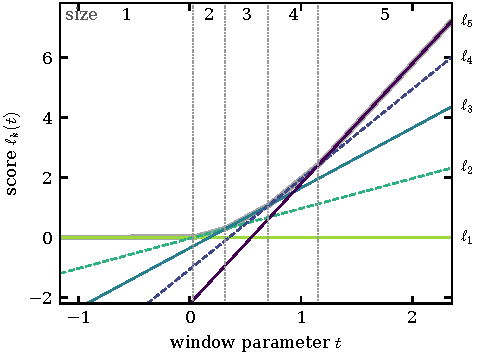
\includegraphics{figures/phases}
\caption{The lines~\eqref{eq:weakfield-lines} for $d=5$ and $h_i=-(i-1)^2$. The
grey band is their upper envelope. The dotted lines are $t_1<\cdots<t_4$, and
the number at the top of each interval is the size $k$ of the winning support
$\{1,\ldots,k\}$.}
\label{fig:phases}
\end{figure}

\begin{remark}[sticky priors]\label{rem:sticky}
Our chain is Paper~C's sticky chain with the uniform kernel. Paper~C normalizes
that chain by $Q=(J-dI)/(d-1)$, so its $T$ and $\tau$ are $d-1$ times ours, and
the tie at our $T=L$ sits at its $\tau=d-1$. The uniform kernel meets Paper~C's
direct-jump criterion with equality for every face. For $d\ge3$ and a symmetric
kernel with all off-diagonal rates positive, Paper~C shows that only the
uniform kernel meets this criterion, so only it ties on every face at first
order. The tie then resolves as a direct jump
(Corollary~\ref{cor:simplex-modes}), while a field
(Corollary~\ref{cor:weakfield-full-hierarchy}) or a start that is not uniform
(Remark~\ref{ex:K3-start}) puts intermediate faces inside the window, of width
$O(1/N)$ in $p$. If the path is observed through a likelihood with
log-likelihood $\langle h,n\rangle/N$, then $\widetilde P_{N,h}$ is the posterior
law of the counts. Kernels that are not uniform act at first order in Paper~C, on
the scale $L$ in $T$, and the field and the start only at order 1, so they are
not interchangeable.
\end{remark}

\begin{remark}[mass versus mode]\label{rem:mass-mode}
From each state of a face $F$ with $k$ states the chain stays in $F$ with
probability $1-(d-k)r$, so $\Prob(\supp K_N\subseteq F)=\mu(F)(1-(d-k)r)^{N-1}$.
So the bins with full support have mass at least
$1-\sum_{|F|=d-1}\mu(F)(1-r)^{N-1}=1-O(e^{-T})$, while for the uniform start,
$t<a_d$ and large $N$ the modes are single states
(Corollary~\ref{cor:simplex-modes}).
\end{remark}


\section{Verification and remaining questions}

The proofs above are analytic and combinatorial. Independent finite
checks are supplied by the standard-library Python scripts accompanying
this draft. The script \texttt{verify\_geometry.py} compares 6,733 exact
rational probabilities in 237 distributions with dynamic programming;
158 distributions also agree with exhaustive enumeration. It checks
normalization, means, covariances, and endpoint parameters for $d=2,3,4$.
The script \texttt{verify\_simplex\_threshold.py} checks the positive
refresh formula, balancing transfers, the finite-size edge-mode example,
and crossing expansions. The scripts
\texttt{verify\_frontier\_boundary.py} and
\texttt{verify\_frontier\_modes.py} check the uniform comparison,
rare-coordinate formulas, spatial profiles, and weak-field assertions
against finite calculations. Finally,
\texttt{verify\_vertex\_completion.py} contains 462 exact identity
comparisons, 200 rational elasticity checks, 16 explicit root-bracket
checks, and four large growing-rare-count stress cases. The associated
records are stored under \texttt{data/}. Decimal asymptotic checks are
numerical corroboration, not interval certificates or substitutes for
the written proofs.

For fixed support size, the leading near-vertex crossing is now uniform
throughout $A=o(b)$. A uniform higher-order expansion throughout that
whole regime remains open here. Other remaining questions include a
growing number of colors, nonuniform switching, and the complete
finite-size mode diagram outside the proved window. The explicit
finite-size edge modes and the divergent probability approximation in
Proposition~\ref{prop:vertex-probability-failure} delimit the results:
they prevent stronger interpretations of the corresponding asymptotic
claims. Before submission, the proposed refinements require independent
mathematical review and completion of the literature comparison.

\begin{thebibliography}{9}
\bibitem{kagey131}
P.~Kagey, \emph{Problem 131}, Open Problem Collection,
\url{https://peterkagey.com/problems/131/} (accessed September 2026).

\bibitem{companion}
A.~Pemmasani, \emph{Endpoint crossings in the persistent random walk:
uniform Bessel bounds and boundary effects}, unpublished companion
manuscript, 2026.

\bibitem{wangyang1995}
Y.~H.~Wang and Z.~J.~Yang, \emph{On a Markov multinomial distribution},
Mathematical Scientist \textbf{20} (1995), 40--49. Bibliographic details
reported through~\cite{wangtang2003}; original text not consulted.

\bibitem{wangtang2003}
Y.~H.~Wang and L.~Tang, \emph{Poisson style convergence theorems for
additive processes defined on Markov chains},
Statistica Sinica \textbf{13} (2003), 227--242.
\url{https://www3.stat.sinica.edu.tw/statistica/oldpdf/A13n114.pdf}.

\bibitem{brydges2007}
D.~Brydges, R.~van der Hofstad and W.~K\"onig,
\emph{Joint density for the local times of continuous-time Markov chains},
Ann.~Probab.~\textbf{35} (2007), 1307--1332.
\url{https://arxiv.org/abs/math/0611525}.

\bibitem{dlmf}
NIST, \emph{Digital Library of Mathematical Functions},
Eqs.~10.25.2 and~10.40.1,
\url{https://dlmf.nist.gov/10.25.E2},
\url{https://dlmf.nist.gov/10.40.E1}.
\end{thebibliography}
\end{document}
